% !TEX root = ../sethomas_thesis_main.tex
\documentclass[border=1mm,
               class=article
               preview]{standalone}
\usepackage{tikz}
\begin{document}
\begin{tikzpicture}
    \pgfmathsetmacro{\xPlexi}{2.5}
    \pgfmathsetmacro{\yPlexi}{1.8}

    % \pgfmathsetmacro{\xSMA}{6.3}
    % \pgfmathsetmacro{\ySMA}{0.7}
    \pgfmathsetmacro{\xSMA}{6.4}
    \pgfmathsetmacro{\ySMA}{2}

    \pgfmathsetmacro{\xPulltester}{0.5}
    \pgfmathsetmacro{\yPulltester}{3.5}

    \node[anchor=south west,inner sep=0] (graph) at (0,0){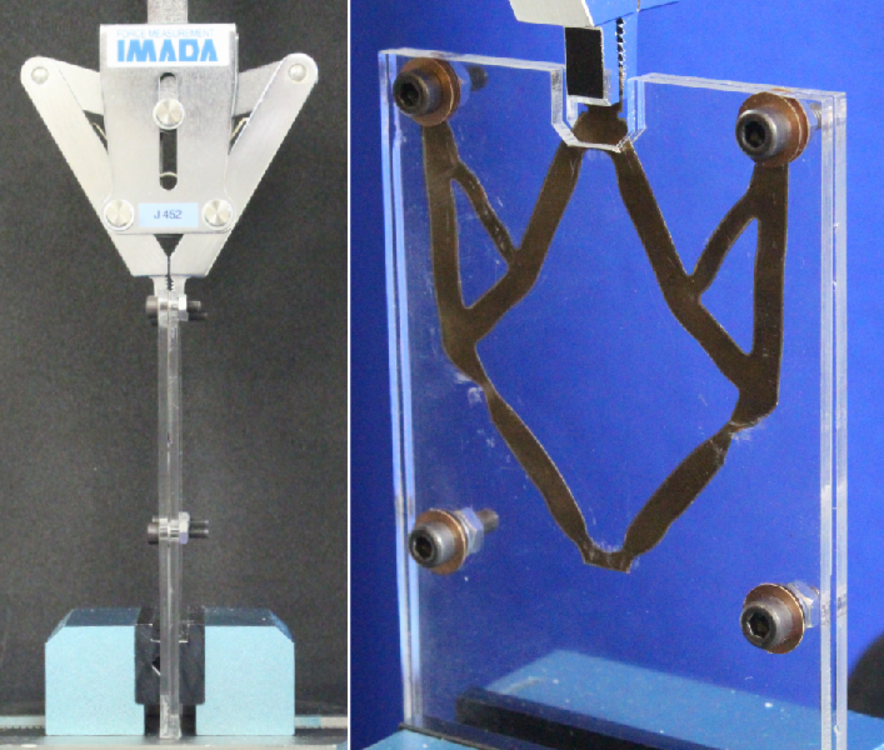
\includegraphics[]{images/chap5/prototype-setup-new5.pdf}};
    \begin{scope}[x={(graph.south east)},y={(graph.north west)}]
        \coordinate (ts0) at (\xPulltester,\yPulltester); \node[align=center] at (ts0) {\color{white}Pull\\\color{white}tester};
        \coordinate (ts1) at (\xPlexi,\yPlexi); \node[align=center] at (ts1) {\color{white}PMMA\\\color{white}plates};
        \coordinate (ts2) at (\xSMA,\ySMA); \node[align=left] at (ts2) {\color{white}SMA};

        \coordinate (SMA_head) at (\xSMA,\ySMA+1.);  \draw[white, thick, -latex](\xSMA,\ySMA+0.25) to (SMA_head);

        \coordinate (PullTester_head) at (\xPulltester+0.3,\yPulltester+1.2);  \draw[white, thick, -latex, bend left](\xPulltester,\yPulltester+0.5) to (PullTester_head);

        \coordinate (plexi_head_1) at (\xPlexi-1.05,\yPlexi+0.9);
        \coordinate (plexi_head_2) at (\xPlexi-0.95,\yPlexi+1.2);
        \coordinate (plexi_head_3) at (\xPlexi+1.4,\yPlexi-0.8);
        \draw[white, thick, -latex, bend right](\xPlexi-0.1,\yPlexi+0.5) to (plexi_head_1);
        \draw[white, thick, -latex,bend right](\xPlexi,\yPlexi+0.5) to (plexi_head_2);
        \draw[white, thick, -latex,bend right](\xPlexi+0.1,\yPlexi-0.5) to (plexi_head_3);

        \draw [-{stealth}{stealth}{stealth}, color=white, ultra thick](5.7,5) --  node[below, sloped] {\color{white}Input} (5.7,6);
        \draw [-{stealth}{stealth}{stealth}, color=white, ultra thick](5.1,1.4) --  node[below, sloped,rotate=180] {\color{white}Output} (5.1,0.4);
    \end{scope}
\end{tikzpicture}%
\end{document}
